\begin{figure}[htbp]
  \centering
  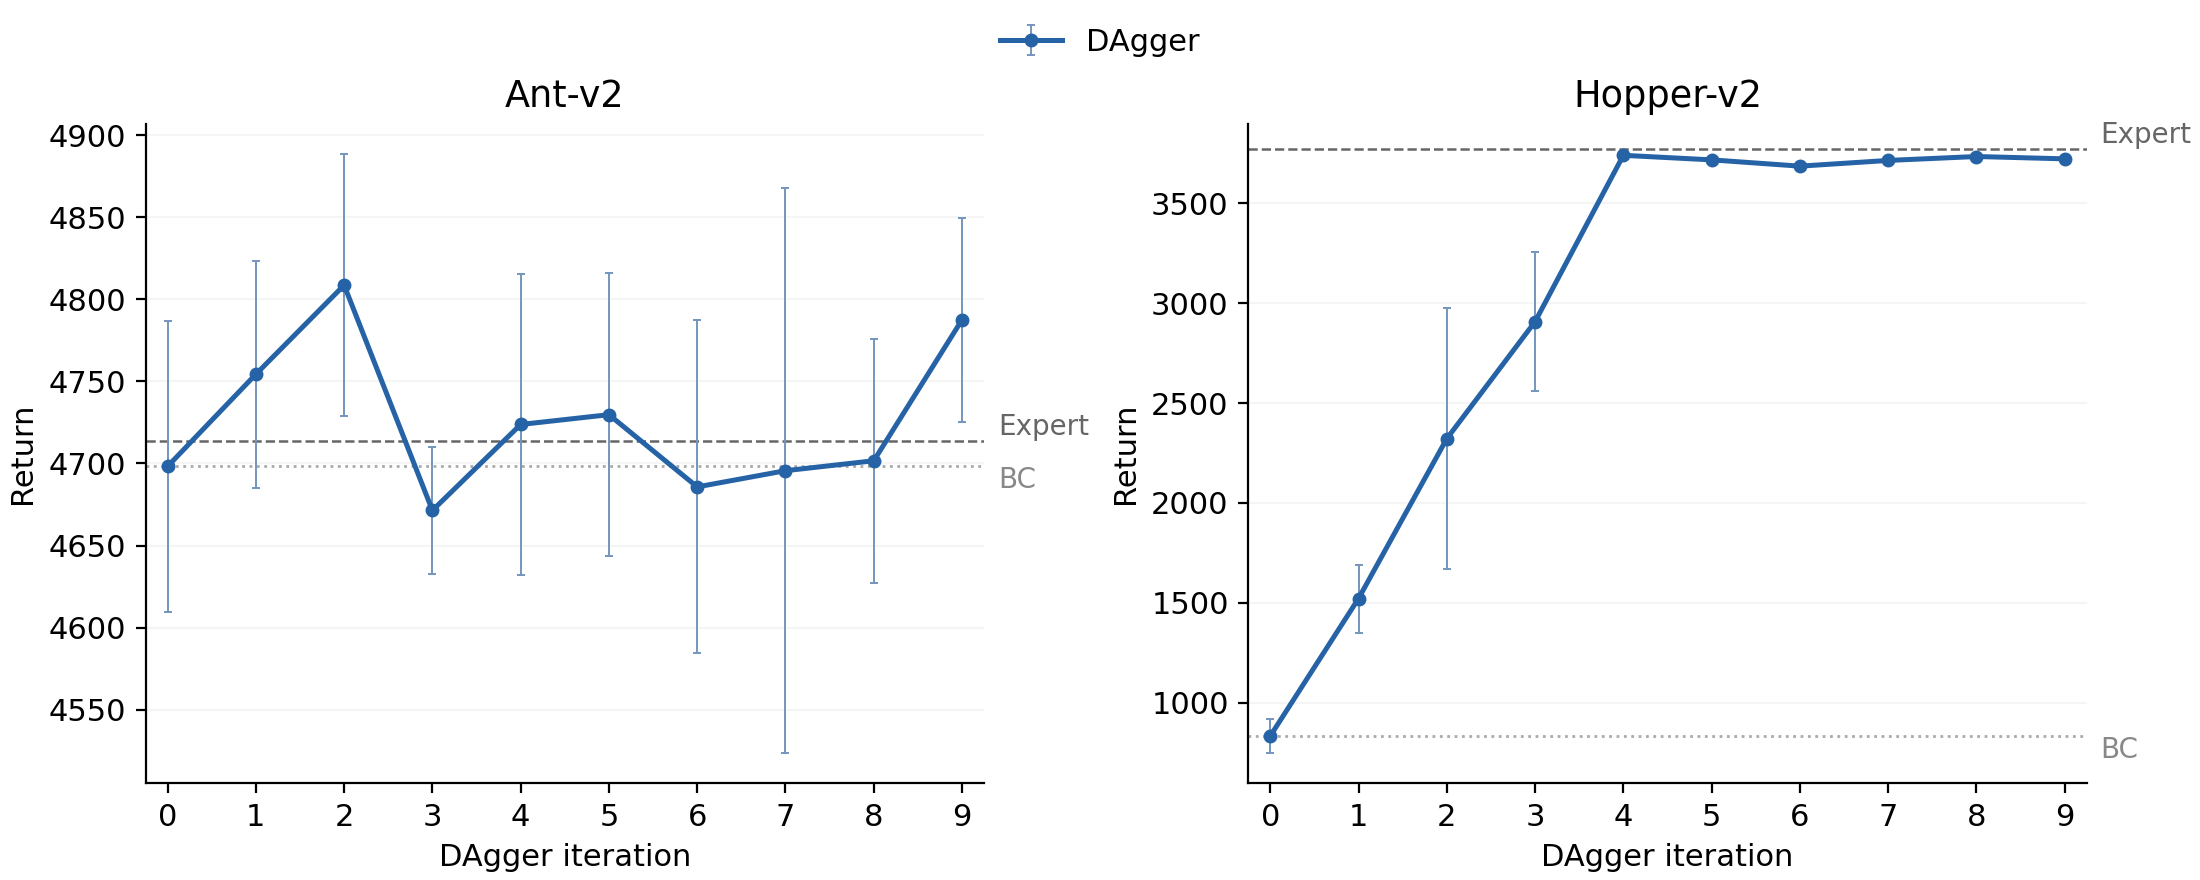
\includegraphics[width=\textwidth]{../results/dagger_comparison/figure2.png}
  \caption{DAgger on Ant-v2 (left) and Hopper-v2 (right). Iteration 0 is BC on two supplied expert trajectories (2,000 transitions); iterations 1--9 each collect at least 1,000 learner transitions in complete episodes, relabel their observations with expert actions, and aggregate them with all previous training data. Policies predict one action using three hidden layers of 64 tanh units and an identity output. Each iteration uses 1,000 Adam updates with MSE loss, learning rate 0.005, and minibatches of 100; seed 1, CPU. These settings match Table 2. Evaluation collects complete episodes until at least 5,000 transitions are reached, with a 1,000-step episode limit (at least five rollouts per point). Points show mean undiscounted episode returns; error bars show population standard deviations, not variation across training seeds. Horizontal lines show the supplied expert demonstrations\textquotesingle{} mean return and the Table 2 BC mean. The panels use different vertical scales. DAgger receives additional expert labels and training updates after iteration 0; the BC reference remains fixed.}
  \label{fig:dagger}
\end{figure}
